\documentclass[pdftex,10pt,xcolor=svgnames]{beamer}

\mode<presentation>
{
  \usetheme{boxes}
  \usecolortheme[named=MidnightBlue]{structure}
  %\setbeamercolor{normal text}{bg=NavajoWhite!20}
  \usefonttheme{serif}
  \setbeamertemplate{navigation symbols}{}
  % Show frame number and author name in footline
  \setbeamertemplate{footline}[frame number]
  \addtobeamertemplate{footline}{\quad\textcolor{gray}{James Robert Lloyd}}{}
  % Set frame titles in small capitals
  \setbeamerfont{frametitle}{shape=\scshape,family=\rmfamily}
  \setbeamercolor{frametitle}{bg=gray!60!white,fg=black}
  % Alerted text: blue (uncomment second line if theme sets alerted text to bold)
  \setbeamercolor{alerted text}{fg=blue}
  %\setbeamerfont*{alerted text}{}
  \setbeamertemplate{bibliography item}[text] %{\hbox{\donotcoloroutermaths$\blacktriangleright$}}
  \setbeamertemplate{bibliography entry title}{}
  \setbeamertemplate{bibliography entry author}{}
  \setbeamertemplate{bibliography entry note}{}
  \setbeamertemplate{bibliography entry location}{}

}
\usepackage[english]{babel}
\usepackage[latin1]{inputenc}
\usepackage{times}
\usepackage[T1]{fontenc}
\usepackage{hyperref}
\usepackage{multimedia}
\usepackage{eepic}
\usepackage{graphicx}
%\usepackage[nohug]{latexinclude/diagrams}
\usepackage{tikz}
\usetikzlibrary{calc}

%% \newcommand{\footlineextra}[1]{
%%     \begin{tikzpicture}[remember picture,overlay]
%%         \node[yshift=1.5ex,anchor=south east] at (current page.south east)
%% {#1};
%%     \end{tikzpicture}
%% }

\newcommand{\footlineextra}[1]{
    \begin{tikzpicture}[remember picture,overlay]
        \node[xshift=-5ex,yshift=-0.5ex,anchor=south east] at (current page.south east)
             {\mbox{\tiny \textcolor{MidnightBlue}{#1}}};
    \end{tikzpicture}
}

\def\sectionframe#1{
  {
    \setbeamertemplate{footline}{\empty}
    \begin{frame}{}
      \begin{center}
        \huge\sc #1
      \end{center}
    \end{frame}
  }
}



\usecolortheme{default}
\xdefinecolor{Black}{rgb}{0,0,0}
\xdefinecolor{White}{rgb}{1,1,1}
\xdefinecolor{DarkBlue}{rgb}{0,0,.7}
\xdefinecolor{DarkRed}{rgb}{.7,0,0}
\xdefinecolor{Red}{rgb}{.85,0,0}
\xdefinecolor{DarkGreen}{rgb}{0,.7,0}
\xdefinecolor{DarkMagenta}{rgb}{.6,0,.6}
\def\Black{\textcolor{Black}}
\def\White{\textcolor{White}}
\def\Blue{\textcolor{DarkBlue}}
\def\Magenta{\textcolor{DarkMagenta}}
\def\Red{\textcolor{Red}}
\def\Green{\textcolor{DarkGreen}}
\definecolor{camlightblue}{rgb}{0.601 , 0.8, 1}

\usepackage{alltt}
\usepackage{psfrag}
\usepackage{pstool}

\def\newarrow{\mbox{\begin{tikzpicture}
             \useasboundingbox{(-3pt,-4.5pt) rectangle (19pt,1pt)};
             \draw[->] (0,-0.07)--(17pt,-0.07);\end{tikzpicture}}}

\title[] % (optional, use only with long paper titles)
{An experiment concerning mathematical writing}

\author % (optional, use only with lots of authors)
{James Robert Lloyd}
% - Use the \inst{?} command only if the authors have different
%   affiliation.

\institute[] % (optional, but mostly needed)
{University of Cambridge}
% - Use the \inst command only if there are several affiliations.
% - Keep it simple, no one is interested in your street address.

\date % (optional)
{May 2013}

\subject{Talks}

\usetikzlibrary{shapes.geometric,arrows,chains,matrix,positioning,scopes}
 \makeatletter
 \tikzset{join/.code=\tikzset{after node path={%
       \ifx\tikzchainprevious\pgfutil@empty\else(\tikzchainprevious)%
       edge[every join]#1(\tikzchaincurrent)\fi}}
 }
 \tikzset{>=stealth',every on chain/.append style={join},
   every join/.style={->}
 }

\tikzstyle{mybox} = [draw=white, rectangle]
\usepackage{ifthen}
\usepackage{booktabs}

% Custom definitions
\def\simiid{\sim_{\mbox{\tiny iid}}}

%%%%%%%%%%%%%%%%%%%%%%%%%%%%%%%%%%%%%%%%%%%%%%%%%%%%%%%%%%
%%%% EDITING HELPER FUNCTIONS  %%%%%%%%%%%%%%%%%%%%%%%%%%%
%%%%%%%%%%%%%%%%%%%%%%%%%%%%%%%%%%%%%%%%%%%%%%%%%%%%%%%%%%

%% NA: needs attention (rough writing whose correctness needs to be verified)
%% TBD: instructions for how to fix a gap ("Describe the propagation by ...")
%% PROBLEM: bug or missing crucial bit 

%% use \fXXX versions of these macros to put additional explanation into a footnote.  
%% The idea is that we don't want to interrupt the flow of the paper or make it 
%% impossible to read because there are a bunch of comments.

%% NA's (and TBDs, those less crucially) should be written so 
%% that they flow with the text.

\definecolor{WowColor}{rgb}{.75,0,.75}
\definecolor{SubtleColor}{rgb}{0,0,.50}

% inline
\newcommand{\NA}[1]{\textcolor{SubtleColor}{ {\tiny \bf ($\star$)} #1}}
\newcommand{\LATER}[1]{\textcolor{SubtleColor}{ {\tiny \bf ($\dagger$)} #1}}
\newcommand{\TBD}[1]{\textcolor{SubtleColor}{ {\tiny \bf (!)} #1}}
\newcommand{\PROBLEM}[1]{\textcolor{WowColor}{ {\bf (!!)} {\bf #1}}}

% as margin notes

\newcounter{margincounter}
\newcommand{\displaycounter}{{\arabic{margincounter}}}
\newcommand{\incdisplaycounter}{{\stepcounter{margincounter}\arabic{margincounter}}}

\newcommand{\fTBD}[1]{\textcolor{SubtleColor}{$\,^{(\incdisplaycounter)}$}\marginpar{\tiny\textcolor{SubtleColor}{ {\tiny $(\displaycounter)$} #1}}}

\newcommand{\fPROBLEM}[1]{\textcolor{WowColor}{$\,^{((\incdisplaycounter))}$}\marginpar{\tiny\textcolor{WowColor}{ {\bf $\mathbf{((\displaycounter))}$} {\bf #1}}}}

\newcommand{\fLATER}[1]{\textcolor{SubtleColor}{$\,^{(\incdisplaycounter\dagger)}$}\marginpar{\tiny\textcolor{SubtleColor}{ {\tiny $(\displaycounter\dagger)$} #1}}}


%% For submission, make all render blank.
%\renewcommand{\LATER}[1]{}
%\renewcommand{\fLATER}[1]{}
%\renewcommand{\TBD}[1]{}
%\renewcommand{\fTBD}[1]{}
%\renewcommand{\PROBLEM}[1]{}
%\renewcommand{\fPROBLEM}[1]{}
%\renewcommand{\NA}[1]{#1}  %% Note, NA's pass through!

%%%%
% Paper specific stuff
%%%%

\newtheorem{thm}{Theorem}%[section]
\newtheorem{lem}[thm]{Lemma}
\newtheorem{prop}[thm]{Proposition}
\newtheorem{cor}[thm]{Corollary}

\newtheorem*{theorem*}{Theorem}

\theoremstyle{definition}
\newtheorem*{definition*}{Definition}
%\newtheorem{definition}[thm]{Definition}%[section]
\newtheorem{conj}{Conjecture}[section]
\newtheorem{exmp}{Example}[section]
\newtheorem{rem}[thm]{Remark}

\theoremstyle{remark}
%\newtheorem{rem}{Remark}
%\newtheorem{note}{Note}
%\newtheorem{case}{Case}

\newcommand{\eqd}{\overset{\,_{\!d}}{=}}
\newcommand{\defn}[1]{\emph{#1}}

\newcommand{\Law}{\mathcal{L}}

\def\given{\,|\,}

\def\SGinf{\mathbb{S}_{\infty}}

\newcommand{\NonNegInts}{\mathbb{Z}_+}
\newcommand{\Nats}{\mathbb{N}}
\newcommand{\Rationals}{\mathbb{Q}}
\newcommand{\Reals}{\mathbb{R}}

\newcommand{\as}{\textrm{a.s.}}

\def\[#1\]{\begin{align}#1\end{align}}
\newcommand{\defas}{:=}

\newcommand{\Normal}{\mathcal{N}}
\newcommand{\dist}{\ \sim\ }

\newcommand{\kernel}{\kappa}
\newcommand{\kernelmatrix}{K}
\newcommand{\scalefactor}{s}
\newcommand{\lengthscale}{\ell}
\newcommand{\targets}{T}
\newcommand{\noise}{\sigma_\targets}
\newcommand{\pseudopoints}{\eta}
\newcommand{\inputpoints}{\xi}
\newcommand{\covhyppar}{\psi}
\newcommand{\logistic}{\phi}

\newcommand{\CompOrder}{\mathcal{O}}
\def\graphspace{\mathbf{G}}
\def\Uniform{\mbox{\rm Uniform}}
\def\Bernoulli{\mbox{\rm Bernoulli}}
\def\ie{i.e.,\ }
\def\eg{e.g.,\ }
\def\iid{i.i.d.\ }
\def\simiid{\sim_{\mbox{\tiny iid}}}
\def\simind{\sim_{\mbox{\tiny ind}}}
\def\eqdist{\stackrel{\mbox{\tiny d}}{=}}
\def\ahfunction{\theta}       
\def\AHfunction{\Theta}           % A-H random function
\def\AHvar{U}                     % A-H uniform variables
\def\AHvaralt{V}                  % A-H uniform variables - for bipartite data
\def\larray{W}                    % latent array sampled with A-H
%\def\latentspace{\mathbf{W}}      % range of entries
\def\latentspace{\mathcal{W}}      % range of entries
\def\darray{X}                    % data array
%\def\dataspace{\mathbf{X}}        % sample space
\def\dataspace{\mathcal{X}}        % sample space
\def\cfspace{\mathbf{C}}          % space of continuous functions
%\def\GP{\mbox{\mathcal{GP}}}
\def\GP{\mathcal{GP}}
\def\likelihood{P}
\def\CovData{C}
\def\CovDataAlt{D}

\begin{document}

\small
%% { 
%%   \setbeamertemplate{footline}{\empty}
%%   \begin{frame}
%%     \titlepage
%%   \end{frame}
%% }
%\renewcommand{\inserttotalframenumber}{11}

%\theoremstyle{plain}

\def\ie{i.e.\ }
\def\eg{e.g.\ }
\def\indicator{\mathbb{I}}
\def\mean#1{\mathbb{E}[#1]}
\def\bigmean#1{\mathbb{E}\bigl[#1\bigr]}
\def\Bigmean#1{\mathbb{E}\Bigl[#1\Bigr]}
\def\cyl{\mathcal{Z}}
\def\eqae{=_{\mbox{\tiny a.e.}}}
\def\wrt{w.r.t.\ }
\def\ae{a.e.\ }
\def\equas{=_{\mbox{\tiny a.s.}}}
\def\equae{=_{\mbox{\tiny a.e.}}}
\def\iid{i.i.d.\ }
\def\Iid{I.i.d.\ }
%\def\inclusion{\jmath}
\def\inclusion{\mathcal{J}}
\def\inclusionX{\inclusion_{\xspace}}
\def\wstar{weak$^{\ast}$ }
% Symmetric difference
\def\symmdiff{\!\vartriangle\!}


% Indices

\def\indI{\mbox{\tiny I}}
\def\indJ{\mbox{\tiny J}}
\def\indK{\mbox{\tiny K}}
\def\indJI{\mbox{\tiny J$\setminus$I}}
\def\indE{\mbox{\tiny E}}
\def\indF{\mbox{\tiny F}}
\def\indD{\mbox{\tiny D}}
\def\indi{\mbox{\tiny{\{i\}}}}
\def\ind#1{\mbox{\tiny #1}}
\def\power{\mathcal{F}}
\def\powerD{\power(D)}
\def\powerE{\power(E)}
\def\powerL{\power(L)}
\def\parts{\mathcal{H}}
\def\partsQ{\parts(\mathcal{Q})}
\def\partsn{\parts[n]}
\def\partsN{\parts_{\infty}(\mathbb{N})}

% Spaces

\def\abstspace{\Omega}
\def\xspace{\mathcal{X}}
\def\yspace{\mathcal{Y}}
\def\tspace{\mathcal{T}}
\def\xspaceI{\xspace_{\indI}}
\def\xspaceJ{\xspace_{\indJ}}
\def\xspaceD{\xspace_{\indD}}
\def\xspaceE{\xspace_{\indE}}
\def\tspaceI{\tspace_{\indI}}
\def\tspaceJ{\tspace_{\indJ}}
\def\tspaceD{\tspace_{\indD}}
\def\tspaceE{\tspace_{\indE}}
\def\txspace{\tilde{\xspace}}
\def\yspaceI{\yspace_{\indI}}
\def\yspaceJ{\yspace_{\indJ}}
\def\yspaceD{\yspace_{\indD}}
\def\yspaceE{\yspace_{\indE}}
\def\txspace{\tilde{\xspace}}
\def\ttspace{\tilde{\tspace}}
\def\xI{x_{\indI}}
\def\xJ{x_{\indJ}}
\def\xD{x_{\indD}}
\def\xE{x_{\indE}}
\def\tImage{\Gamma}
\def\simp{\triangle}
\def\simpI{\simp_{\indI}}
\def\simpJ{\simp_{\indJ}}

\def\AI{A_{\indI}}
\def\AJ{A_{\indJ}}
\def\AD{A_{\indD}}
\def\AE{A_{\indE}}


%Space of Prob Measures
\def\pMeas{M}
%Space of Contents
\def\fMeas{N}
%Space of cont fcts
\def\cfspace{C}
%Hilbert space
\def\hilbert{\mathcal{L}^2}


\def\borelV{\borel_{V}}

% Set systems

\def\borel{\mathcal{B}}
\def\top{\mbox{Top}}

\def\borelI{\borel_{\indI}}
\def\borelJ{\borel_{\indJ}}
\def\borelD{\borel_{\indD}}
\def\borelE{\borel_{\indE}}
\def\tborel{\tilde{\borel}}
\def\abstfield{\mathcal{A}}
\def\field{\mathcal{C}}
\def\fieldI{\field_{\indI}}
\def\fieldJ{\field_{\indJ}}
\def\fieldK{\field_{\indK}}
\def\fieldD{\field_{\indD}}
\def\fieldE{\field_{\indE}}
\def\tfield{\tilde{\mathcal{C}}}
\def\Sfield{\mathcal{S}}
\def\SfieldI{\mathcal{S}_{\indI}}
\def\SfieldJ{\mathcal{S}_{\indJ}}
\def\SfieldD{\mathcal{S}_{\indD}}
\def\tSfield{\tilde{\mathcal{S}}}
\def\borelx{\borel_x}
\def\tborelx{\tborel_x}
\def\borelgamma{\tborel_{\tImage}}
%\def\borelth{\borel_{\theta}}
\def\borely{\borel_{y}}
%\def\borelT{\borel_t}
\def\borelT{\borel_{\tspace}}
\def\borelS{\borel_s}
\def\topI{\top_{\indI}}
\def\topJ{\top_{\indJ}}
\def\topD{\top_{\indD}}
\def\topE{\top_{\indE}}
\def\topV{\top_V}
\def\topws{\top_{\text{ws}}}
\def\topcc{\top_{\text{c}}}
\def\borelXI{\borel(\xspaceI)}
\def\borelXD{\borel(\xspaceD)}
\def\tborelX{\borel(\txspace)}
\def\borelTI{\borel(\tspaceI)}
\def\borelTD{\borel(\tspaceD)}
\def\tborelT{\borel(\ttspace)}


% Maps

\def\XI{X_{\indI}}
\def\Xi{X_{\ind{i}}}
\def\Xj{X_{\ind{j}}}
\def\ThetaI{\Theta_{\indI}}
\def\XJ{X_{\indJ}}
\def\ThetaJ{\Theta_{\indJ}}
\def\XD{X_{\indD}}
\def\ThetaD{\Theta_{\indD}}
\def\XE{X_{\indE}}
\def\ThetaE{\Theta_{\indE}}
\def\tX{\tilde{X}}
\def\tTheta{\tilde{\Theta}}

\def\SI{S_{\indI}}
\def\TI{T_{\indI}}

\def\rest{\phi}
\def\restD{\rest_{\indD}}
\def\restI{\rest_{\indI}}
\def\restJ{\rest_{\indJ}}
\def\restDI{\rest^{\indD}_{\indI}}
\def\inclusionD{\inclusion_{\indD}}
\def\inclusionE{\inclusion_{\indE}}
\def\projector{\mbox{pr}}
\def\projectorD{\projector_{\indD}}
\def\projectorI{\projector_{\indI}}
\def\projectorJI{\pi_{\indJ\indI}}
\def\indicator{\mathbb{I}}

% Projective systems

\def\po{\preceq}
\def\famD#1{{\lbrace #1 \rbrace}_{\indD}}
\def\famE#1{{\lbrace #1 \rbrace}_{\ind{I$\in$}\indE}}
\def\fJI{f_{\indJ\indI}}
\def\fKI{f_{\indK\indI}}
\def\fKJ{f_{\indK\indJ}}
\def\fII{f_{\indI\indI}}
\def\fI{f_{\indI}}
\def\fJ{f_{\indJ}}
\def\fK{f_{\indK}}
\def\fD{f_{\indD}}
\def\fDI{f^{\indD}_{\indI}}
\def\fDK{f^{\indD}_{\indK}}
\def\gJI{g_{\indJ\indI}}
\def\gI{g_{\indI}}
\def\gJ{g_{\indJ}}
\def\gD{g_{\indD}}
\def\hJI{h_{\indJ\indI}}
\def\hI{h_{\indI}}
\def\hJ{h_{\indJ}}
\def\hE{h_{\indE}}
\def\plim{\varprojlim}

% Measure and Conditionals

\def\abstmeasure{\mathbb{P}}
\def\P{P}
\def\PI{P_{\indI}}
\def\PJ{P_{\indJ}}
\def\PD{P_{\indD}}
\def\PE{P_{\indE}}
\def\PX{P_{\mbox{X}}}
\def\PTh{P_{\mbox{\Theta}}}
\def\PXI{P_{\XI}}
\def\PThI{P_{\mbox{\Theta}}}
\def\PXJ{P_{\mbox{X}}}
\def\PThJ{P_{\mbox{\Theta}}}
\def\PXD{P_{\mbox{X}}}
\def\PThD{P_{\mbox{\Theta}}}
\def\PXE{P_{\mbox{X}}}
\def\PThE{P_{\mbox{\Theta}}}
\def\tP{\tilde{P}}
\def\tPX{\tilde{P}_X}
\def\tPTh{\tilde{P}_{\Theta}}







\def\SI{S_{\indI}}
\def\SJ{S_{\indJ}}

\def\tk{\tilde{k}}
\def\kI{k_{\indI}}

\def\postkernel{k}
\def\indctr{\mathbbm{1}}
\def\sp#1{\left<#1\right>}


%Mallows
\def\Sr{\mathbb{S}_r}
\def\Sinf{\mathbb{S}_{\infty}}
\def\Sbar{\bar{\mathbb{S}}}
\def\DP#1{\mbox{DP}\left( #1 \right)}
\def\GP#1{\mbox{GP}\left( #1 \right)}
\def\x{\mathbf{x}}
\def\y{\mathbf{y}}



\def\tyspace{\tilde{\yspace}}
\def\tF{\tilde{F}}
\def\tT{\tilde{T}}
\def\tmodel{\tilde{\model}}
\def\tnu{\tilde{\nu}}


\def\PTheta{P^{\theta}}
\def\FTheta{F^{\theta}}
\def\TTheta{T^{\theta}}
\def\borelY{\borel_{\yspace}}

\def\PX{P^{x}}
\def\PXI{\PX_{\indI}}
\def\PXJ{\PX_{\indJ}}
\def\PXD{\PX_{\indD}}
\def\PThetaI{\PTheta_{\indI}}
\def\PThetaD{\PTheta_{\indD}}
\def\YI{Y_{\indI}}
\def\YJ{Y_{\indJ}}
\def\YD{Y_{\indD}}
\def\Tn{T^{(n)}}
\def\indexspace{\mathcal{W}}
\def\tyspace{\tilde{\yspace}}
\def\tY{\tilde{Y}}
\def\inclusionT{\inclusion_{\tspace}}
\def\tPTheta{\tilde{P}^{\theta}}
\def\tTn{\tilde{T}^{(n)}}
\def\inclusionY{\inclusion_{\yspace}}

\def\tyspace{\tilde{\yspace}}
\def\tF{\tilde{F}}
\def\tT{\tilde{T}}
\def\tmodel{\tilde{\model}}
\def\tnu{\tilde{\nu}}
\def\tOmega{\tilde{\abstspace}}
\def\tabstmeasure{\tilde{\abstmeasure}}
\def\model{\mathcal{P}}

\def\tf{\tilde{f}}
\def\tx{\tilde{x}}
\def\Dom{\mbox{Dom}}
\def\ty{\tilde{y}}


\begin{frame}
  \begin{block}{}
    \titlepage
  \end{block}
\end{frame}

\begin{frame}{Spot the odd one out (not the proposition)}
  \begin{block}{Proposition}
Let $X$ be a complete metric space and let $A$ be a closed subset of $X$. Then $A$ is complete.
  \end{block}
  \begin{block}{Proof 1}
Consider an arbitrary Cauchy sequence $(x_n)_{\{n\in\Nats\}}$ in $A$. As $X$ is complete, $(x_n)$ has a limit in $X$. Suppose $\lim_{n\to\infty} = x$. Because $A$ is closed, $x$ belongs to $A$. We've proved that every Cauchy sequence in $A$ has a limit point in $A$. So $A$ is complete.
  \end{block}
  \begin{block}{Proof 2}
Let $(a_n)$ be a Cauchy sequence in $A$. Then, since $X$ is complete, we have that $(a_n)$ converges. That is, there exists $a$ such that $a_n \to a$. Since $A$ is closed in $X$, $(a_n)$, is a sequence in $A$ and $a_n \to a$, we have that $a \in A$. Thus $(a_n)$ converges in $A$ and we are done.
  \end{block}
  \begin{block}{Proof 3}
Let $(a_n)$ be a Cauchy sequence in $A$. We want to show that $(a_n)$ tends to a limit in $A$. Siunce $A$ is a subset of $X$, $(a_n)$ is a Cauchy sequence in $X$. Since $X$ is complete, $a_n \to a$, for some $a \in X$. Since $A$ is a closed subset of $X$, it must contain all its limit points, so $a \in A$. So $a_n \to a$ in $A$. So $A$ is complete.
  \end{block}
\end{frame}

\begin{frame}{A mathematical writing Turing test}
  \begin{block}{Computer identified 50\% of the time}
    \begin{center}
      \begin{tikzpicture}
  \begin{scope}[yshift=0cm]
    \begin{scope}[xshift=0cm]
      \node [mybox] (box){
        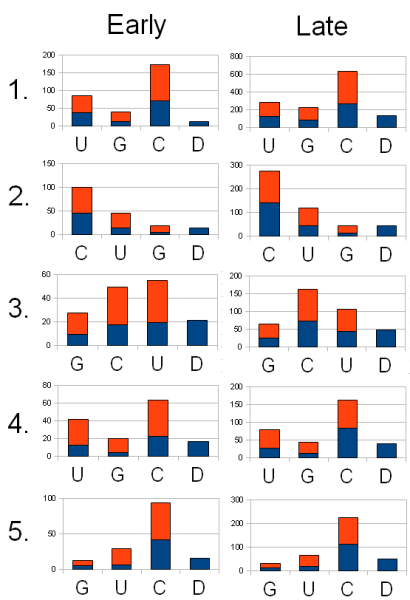
\includegraphics[width=0.35\textwidth]{../figures/whichisthecomputer.png}
      };
    \end{scope}
  \end{scope}
  \begin{scope}[yshift=0.15\textwidth]
    \begin{scope}[xshift=0.5\textwidth]
      \node [mybox] (box) [text width=0.5\textwidth]{
        This talk is based on the current latest blog post by Tim Gowers
      };
    \end{scope}
  \end{scope}
  \begin{scope}[yshift=0.0\textwidth]
    \begin{scope}[xshift=0.5\textwidth]
      \node [mybox] (box) [text width=0.5\textwidth]{
        Results taken after revealing that one solution was produced by a computer
      };
    \end{scope}
  \end{scope}
  \begin{scope}[yshift=-0.15\textwidth]
    \begin{scope}[xshift=0.5\textwidth]
      \node [mybox] (box) [text width=0.5\textwidth]{
        Computer identified $\sim50\%$ of the time, but undergraduate a strong contender
      };
    \end{scope}
  \end{scope}
\end{tikzpicture}

    \end{center}
  \end{block}
\end{frame}

\begin{frame}{Aims and purpose of the system}
  \begin{itemize}
    \item The program should not find a step hard if an experienced human finds it obvious.
    \vspace{2\baselineskip}
    \item The program should not be willing to do a step if an experienced human would be very reluctant to do it.
    \vspace{2\baselineskip}
    \item The methods that the program uses should not be specific to any domain of mathematics. Any domain specific behaviour should be the result of data that the program is given to work with.
  \end{itemize}
\end{frame}

\begin{frame}{A very brief description of the program}
  \begin{itemize}
    \item Natural language input parsed into list of assumed statements (hypotheses) and target statements
    \vspace{1\baselineskip}
    \item A list of rules is applied to the statements greedily, picking the first that can be applied
    \begin{itemize}
      \item Scope and order of rules is one of the main intellectual contributions of the work
      \item Designed to give the desired human like behaviour
    \end{itemize}
    \vspace{1\baselineskip}
    \item Each rule applied generates a sentence in the proof
    \begin{itemize}
      \item If the rules, and the ways of applying them, are sufficiently `human' then the output should resemble a stream of conciousness from a mathematician
    \end{itemize}
  \end{itemize}
\end{frame}

\begin{frame}{Worked example}
  \begin{block}{Proposition}
Let $X$ and $Y$ be metric spaces, let $f : X \to Y$ be continuous, and let $U$ be an open subset of $Y$.
Then $f^{-1}(U)$ is an open subset of $X$.
  \end{block}
  \vspace{3\baselineskip}
  \begin{block}{Automatically constructed proof}
Let $x$ be an element of $f^{-1}(U)$. Then $f(x) \in U$. Therefore, since $U$ is open, there exists $\eta > 0$ such that $u \in U$ whenever $d(f(x), u) < \eta$. We would like to find $\delta > 0$ s.t.\ $y \in f^{-1}(U)$ whenever $d(x, y) < \delta$. But $y \in f^{-1}(U)$ if and only if $f(y) \in U$. We know that $f(y) \in U$ whenever $d(f(x), f(y)) < \eta$. Since $f$ is continuous, there exists $\theta > 0$ such that $d(f(x), f(y)) < \eta$ whenever $d(x, y) < \theta$. Therefore, setting $\delta = \theta$, we are done.
  \end{block}
\end{frame}

\begin{frame}{Worked example\ldots}
  \begin{block}{Hypotheses}
    \begin{itemize}
      \item $f$ is continuous
      \item $U$ is open
    \end{itemize}
  \end{block}
  \begin{block}{Targets}
    \begin{itemize}
      \item $f^{-1}(U)$ is open
    \end{itemize}
  \end{block}
  \begin{block}{}
    Input to program after parsing problem.
    Also has `background' information \eg $X$, $Y$ are metric spaces, $f : X \to Y$ etc.
  \end{block}
\end{frame}

\begin{frame}{Worked example\ldots}
  \begin{block}{Hypotheses}
    \begin{itemize}
      \item $f$ is continuous
      \item $U$ is open
      \item $x \in f^{-1}(U)$
    \end{itemize}
  \end{block}
  \begin{block}{Targets}
    \begin{itemize}
      \item $\exists\,\delta\,\forall\,y\quad d(x, y) < \delta \implies y \in f^{-1}(U)$
    \end{itemize}
  \end{block}
  \begin{block}{}
    Convert target into lower-level language
  \end{block}
\end{frame}

\begin{frame}{Worked example\ldots}
  \begin{block}{Hypotheses}
    \begin{itemize}
      \item $f$ is continuous
      \item $U$ is open
      \item $f(x) \in U$
    \end{itemize}
  \end{block}
  \begin{block}{Targets}
    \begin{itemize}
      \item $\exists\,\delta\,\forall\,y\quad d(x, y) < \delta \implies y \in f^{-1}(U)$
    \end{itemize}
  \end{block}
  \begin{block}{}
    Rewrite of inverse statement
  \end{block}
\end{frame}

\begin{frame}{Worked example\ldots}
  \begin{block}{Hypotheses}
    \begin{itemize}
      \item $f$ is continuous
      \item $\forall\,u\quad d(f(x), u) < \eta \implies u \in U$
    \end{itemize}
  \end{block}
  \begin{block}{Targets}
    \begin{itemize}
      \item $\exists\,\delta\,\forall\,y\quad d(x, y) < \delta \implies y \in f^{-1}(U)$
    \end{itemize}
  \end{block}
  \begin{block}{}
    `$f(x) \in U$' is the type of statement that can be provided as input to `$U$ is open'
  \end{block}
\end{frame}

\begin{frame}{Worked example\ldots}
  \begin{block}{Hypotheses}
    \begin{itemize}
      \item $f$ is continuous
      \item $\forall\,u\quad d(f(x), u) < \eta \implies u \in U$
    \end{itemize}
  \end{block}
  \begin{block}{Targets}
    \begin{itemize}
      \item $\forall\,y\quad d(x, y) < \delta^\bullet \implies y \in f^{-1}(U)$
    \end{itemize}
  \end{block}
  \begin{block}{}
    No trivial operations available, temporarily assume $\delta$ is known
  \end{block}
\end{frame}

\begin{frame}{Worked example\ldots}
  \begin{block}{Hypotheses}
    \begin{itemize}
      \item $f$ is continuous
      \item $\forall\,u\quad d(f(x), u) < \eta \implies u \in U$
      \item $d(x, y) < \delta^\bullet[\bar{y}]$
    \end{itemize}
  \end{block}
  \begin{block}{Targets}
    \begin{itemize}
      \item $y \in f^{-1}(U)$
    \end{itemize}
  \end{block}
  \begin{block}{}
    The target can now be split, remembering that $\delta$ cannot depend on $y$
  \end{block}
\end{frame}

\begin{frame}{Worked example\ldots}
  \begin{block}{Hypotheses}
    \begin{itemize}
      \item $f$ is continuous
      \item $\forall\,u\quad d(f(x), u) < \eta \implies u \in U$
      \item $d(x, y) < \delta^\bullet[\bar{y}]$
    \end{itemize}
  \end{block}
  \begin{block}{Targets}
    \begin{itemize}
      \item $f(y) \in U$
    \end{itemize}
  \end{block}
  \begin{block}{}
    Rewrite of inverse statement
  \end{block}
\end{frame}

\begin{frame}{Worked example\ldots}
  \begin{block}{Hypotheses}
    \begin{itemize}
      \item $f$ is continuous
      \item $d(x, y) < \delta^\bullet[\bar{y}]$
    \end{itemize}
  \end{block}
  \begin{block}{Targets}
    \begin{itemize}
      \item $d(f(x), f(y)) < \eta$
    \end{itemize}
  \end{block}
  \begin{block}{}
    Replacement of target $Q(x)$ with $P(x)$ whenever there is a hypothesis $\forall\,u\,\,P(u) \implies Q(u)$
  \end{block}
\end{frame}

\begin{frame}{Worked example\ldots}
  \begin{block}{Hypotheses}
    \begin{itemize}
      \item $d(x, y) < \delta^\bullet[\bar{y}]$
    \end{itemize}
  \end{block}
  \begin{block}{Targets}
    \begin{itemize}
      \item $d(x, y) < \theta[x, \eta]$
    \end{itemize}
  \end{block}
  \begin{block}{}
    Continuity of $f$ can be applied to the target in its current form. $\theta$ noted to depend on $x$ and $\eta$.
  \end{block}
\end{frame}

\begin{frame}{Points for discussion}
  \begin{itemize}
    \item Should we try to make computers think like mathematicians?
    \vspace{2\baselineskip}
    \item Will this constraint always result in sub-state-of-the-art theorem prooving?
    \vspace{2\baselineskip}
    \item Can a system learn how to think like a mathematician, as opposed to a Cambridge senior wrangler polymath designing the system?
    \vspace{2\baselineskip}
    \item \ldots
  \end{itemize}
\end{frame}

\end{document}


